Las Figuras \ref{Fig: simple}-\ref{Fig: ridge} muestran las predicciones de los modelos de regresión implementados, dichas predicciones se realizaron tanto en el conjunto de prueba con en el conjunto de desarrollo.

De forma general se observan predicciones acertadas, pero al revisar con detalle las métricas obtenidas para cada modelo de regresión (Tabla \ref{Tab: results}) se puede observar claramente que el modelo que obtuvo predicciones más cercanas a la realidad fue el modelo de regresión lineal múltiple (Figura \ref{Fig: multiple}).

Una consideración importante también es el grado del polinomio de la regresión polinomial (Figura \ref{Fig: polinomial}) se implementó considerando un grado 2, lo cuál puede generar que se disminuya su desempeño pero a su vez previene el sobre-entrenamiento.

\begin{table}[H]
\centering
\caption{Comparación de métricas de desempeño para cada modelo de regresión.}
\begin{tabular}{@{}lllllll@{}}
\toprule
Algoritmo de regresión & MSE  & RMSE & MAE  & RSE  & PCC  & R2   \\ \midrule
Lineal simple          & 2.71 & 1.65 & 1.28 & 0.08 & 0.98 & 0.92 \\
Polinomial             & 8.22 & 2.87 & 2.40 & 0.24 & 0.97 & 0.76 \\
Lineal múltiple        & 0.33 & 0.57 & 0.49 & 0.01 & 1.00 & 0.99 \\
Ridge                  & 0.64 & 0.80 & 0.60 & 0.02 & 0.99 & 0.98 \\ \bottomrule
\end{tabular}
\label{Tab: results}
\end{table}

\newpage

\begin{figure}[t]
	\centering
	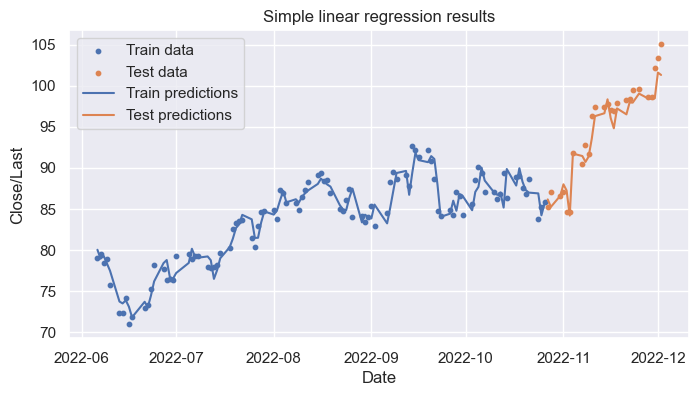
\includegraphics[width=0.8\textwidth]{simple_linear_regression_results}
	\caption{Resultados de regresión lineal simple.}
	\label{Fig: simple}
\end{figure}

\begin{figure}[b]
	\centering
	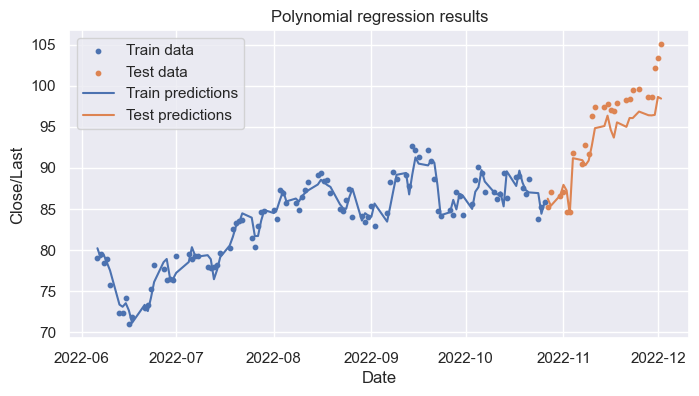
\includegraphics[width=0.8\textwidth]{polynomial_regression_results}
	\caption{Resultados de regresión polinomial.}
	\label{Fig: polinomial}
\end{figure}

\begin{figure}[b]
	\centering
	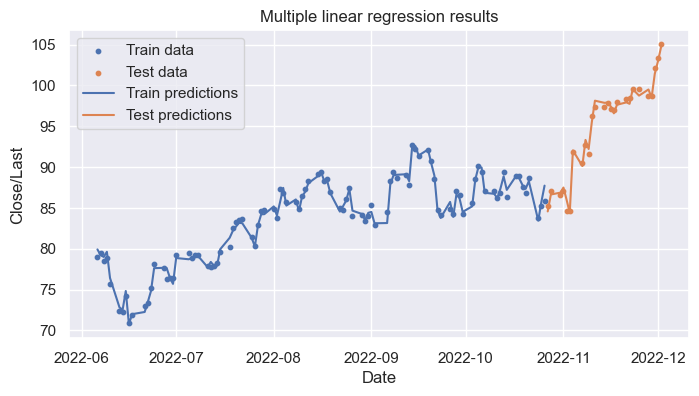
\includegraphics[width=0.8\textwidth]{multiple_linear_regression_results}
	\caption{Resultados de regresión lineal multiple.}
	\label{Fig: multiple}
\end{figure}

\begin{figure}[t]
	\centering
	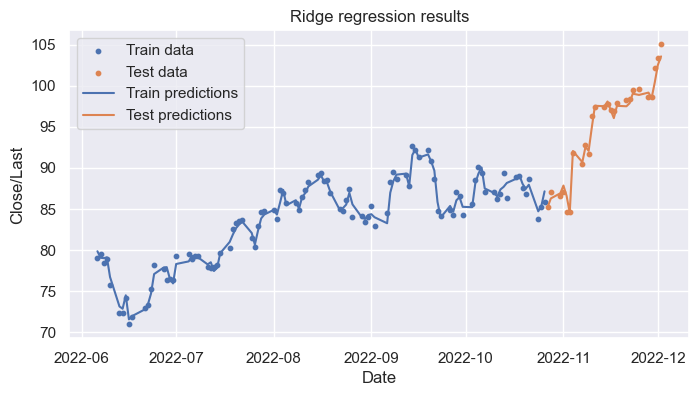
\includegraphics[width=0.8\textwidth]{ridge_regression_results}
	\caption{Resultados de regresión Ridge.}
	\label{Fig: ridge}
\end{figure}
